\documentclass[conference,a4paper]{IEEEtran}
\IEEEoverridecommandlockouts
\usepackage[T1]{fontenc}
\usepackage[utf8]{inputenc}
\usepackage[spanish,es-tabla,es-nodecimaldot]{babel}
\usepackage{newtxtext,newtxmath}
\usepackage{icomma}
\usepackage{amsmath}
\usepackage{booktabs}
\usepackage{array}
\usepackage{multirow}
\usepackage{graphicx}
\usepackage{xcolor}
\usepackage{pgfplots}
\pgfplotsset{compat=1.18}
\usepgfplotslibrary{fillbetween}
\usetikzlibrary{babel,arrows.meta,calc}
\usepackage{url}
\usepackage[hidelinks]{hyperref}

\definecolor{accent}{HTML}{0E6F7C}
\definecolor{warm}{HTML}{C2511A}
\definecolor{muted}{HTML}{6B7280}
\definecolor{ink}{HTML}{1F2937}

\pgfplotsset{informe/.style={
  width=\columnwidth, height=5.2cm,
  tick label style={font=\scriptsize}, label style={font=\footnotesize},
  legend style={font=\scriptsize,draw=none,fill=none},
  axis lines=left, grid=major, grid style={gray!20},
  /pgf/number format/use comma}}

\begin{document}

\title{Replicación independiente de la validación de FAST-LoRa: cuánto del error es del modelo y cuánto del simulador}

\author{\IEEEauthorblockN{Matias Perez Nieto}
\IEEEauthorblockA{Departamento de Electrónica\\
Universidad Técnica Federico Santa María\\
Chile}}

\maketitle

\begin{abstract}
FAST-LoRa es un modelo analítico que calcula, sin simular paquete a paquete, la razón de entrega de paquetes (PDR) y la eficiencia energética (EE) de cada nodo de una red LoRaWAN. Sus autores lo compararon con el simulador FLoRa y reportan un error absoluto medio (MAE) de 0,940$\times10^{-2}$ en la PDR y de 0,040~bits/mJ en la EE. Este trabajo repite esa validación con el código, la copia de FLoRa y los datos crudos de los autores, que se recuperaron del historial de su repositorio. El entorno reproduce sus resultados de forma exacta, y las Tablas~6 y~7 del artículo coinciden celda por celda. Como los autores corrieron FLoRa una sola vez por red, se agregaron cuatro corridas con otras semillas a cada una de sus 80 redes. Con una corrida, el 88~\% del MAE de la PDR se explica por el azar propio de FLoRa. Promediando cinco corridas, en redes de hasta 100 nodos el error del modelo queda entre 0,36 y 0,37$\times10^{-2}$, igual al piso que impone ese azar, mientras que con 500 nodos el modelo subestima la PDR de forma sistemática en 0,2 a 0,5$\times10^{-2}$. El error de la EE se debe casi entero a que cada herramienta usa otro tiempo en el aire y otra potencia de transmisión: con todos los parámetros iguales a los de FLoRa y cinco corridas por red, el MAE baja de 0,040 a 0,009~bits/mJ. La aceleración medida es de 1,5 a 3,3$\times10^{4}$, un orden de magnitud más que lo que dice el texto del artículo.
\end{abstract}

\begin{IEEEkeywords}
LoRaWAN, FLoRa, modelo analítico, PDR, eficiencia energética, reproducibilidad.
\end{IEEEkeywords}

\section{Introducción}

Una red LoRaWAN (\emph{Long Range Wide Area Network}) conecta sensores alimentados con baterías, que aquí se llaman nodos, con antenas receptoras llamadas gateways, a distancias de varios kilómetros. Los nodos transmiten cuando tienen un dato, sin coordinarse entre sí, y cada uno usa dos parámetros de radio. El factor de ensanchamiento (SF, \emph{spreading factor}) es un entero entre 7 y 12: cada paso duplica la duración del paquete y le permite llegar más lejos. La potencia de transmisión va de 2 a 16~dBm. Un SF alto ocupa más tiempo el canal y aumenta los choques con otros nodos, y una potencia alta acorta la vida de la batería. Con 6 SF y 8 potencias hay 48 combinaciones por nodo, y con 100 nodos unas $10^{168}$ configuraciones de red. Elegir una buena exige evaluar muchas, ya sea con una búsqueda o entrenando agentes de aprendizaje por refuerzo.

La forma habitual de evaluar una configuración es un simulador de eventos discretos como FLoRa~\cite{flora}, que genera cada paquete, sortea cuánto se atenúa en el camino y revisa si choca con otro. El resultado es detallado, pero lento: según la Fig.~6 de~\cite{fastlora}, simular 200 nodos durante 5 días toma más de 5~minutos. FAST-LoRa~\cite{fastlora} reemplaza esa simulación por fórmulas de probabilidad y entrega en milisegundos la razón de entrega de paquetes (PDR, \emph{Packet Delivery Ratio}) y la eficiencia energética (EE, bits útiles entregados por unidad de energía) de todos los nodos. Sus autores lo compararon con FLoRa y reportan un error absoluto medio (MAE, \emph{Mean Absolute Error}) de 0,940$\times10^{-2}$ en la PDR y de 0,040~bits/mJ en la EE.

Un modelo así se usa precisamente para no simular, de modo que si se equivoca en algún tipo de red, las configuraciones que se optimicen con él heredan el error sin que nadie lo note. Hasta octubre de 2026 el artículo tenía cuatro citas, tres del mismo grupo, y ninguna repetía la validación. Esa validación tiene puntos débiles que el artículo no muestra. Se hizo contra una copia de FLoRa modificada por los autores, con una sola corrida del simulador por red y sin informar el tamaño del paquete. La corrida única importa porque FLoRa también tiene azar: la PDR que mide es una proporción sobre unos 432 paquetes por nodo, y su error de muestreo es del mismo orden que el MAE reportado. Con los datos publicados no se puede saber qué parte de ese MAE es error del modelo.

Este trabajo repite la validación de forma independiente para responder esa pregunta. Se montó el entorno de los autores en un contenedor, se recuperaron sus datos crudos y se reprodujeron sus resultados de forma exacta. Luego se agregaron cuatro corridas de FLoRa con semillas distintas a cada una de sus 80 redes y se midió por separado el efecto de cada diferencia encontrada entre el artículo, el código del modelo y FLoRa. Hasta 100 nodos el modelo resulta tan exacto como FLoRa permite medir. Con 500 nodos tiene un sesgo pequeño y persistente, y el error de la EE viene sobre todo de que ambas herramientas usan parámetros distintos.

\section{Trabajos relacionados}

Las herramientas para evaluar redes LoRa se pueden ordenar según cuánto detalle modelan. En un extremo están los análisis de la red completa. El de ALOHA puro~\cite{abramson}, el acceso sin coordinación que usa LoRaWAN, da un aprovechamiento máximo del canal de $1/(2e)\approx18$~\%, y Georgiou y Raza~\cite{georgiou} usan geometría estocástica para obtener la cobertura de un gateway en función de la densidad de nodos. Ambos entregan promedios de la red y no sirven para decidir el SF de un nodo en particular.

En el otro extremo están los simuladores que generan cada paquete. LoRaSim~\cite{bor} introdujo el modelo de propagación cuyos parámetros usa también FAST-LoRa. Magrin et al.~\cite{magrin} y Van den Abeele et al.~\cite{vandenabeele} desarrollaron módulos para ns-3, y el segundo mostró que el análisis de ALOHA subestima la capacidad porque ignora el efecto captura, por el que el paquete más fuerte sobrevive a un choque. FLoRa~\cite{flora} corre sobre el simulador OMNeT++ y su biblioteca de modelos de red INET, modela el consumo de la radio por estado y es la referencia de~\cite{fastlora}. Croce et al.~\cite{croce} midieron que los SF no son del todo ortogonales y entregaron la matriz de umbrales de captura que usan FLoRa y FAST-LoRa.

Entre ambos están los modelos por dispositivo. Toro-Betancur et al.~\cite{toro} calculan la probabilidad de entrega de cada nodo según su distancia, su SF y la interferencia de los demás, y Zhang et al.~\cite{zhang} usan una formulación parecida como entorno para entrenar agentes de aprendizaje por refuerzo. FAST-LoRa toma de~\cite{zhang} la separación de la PDR en un término de cobertura y otro de interferencia, y agrega la recepción por varios gateways, la EE y el consumo medido por Liando et al.~\cite{liando}. El aporte de este trabajo está en revisar la validación de ese modelo. Cualquier error medido aquí vale para el entorno de propagación de~\cite{bor}: Lima et al.~\cite{lima}, por ejemplo, obtuvieron otros parámetros en la Amazonía.

\section{Cómo calcula FAST-LoRa y cómo mide FLoRa}
\label{sec:modelo}

Un paquete LoRa se pierde por una de dos razones: llega demasiado débil al gateway o choca con el de otro nodo. FAST-LoRa calcula la probabilidad de cada una para todos los pares nodo-gateway. Esta sección resume sus ecuaciones y señala dónde aparece cada una en el artículo original.

\subsection{Tiempo en el aire}

LoRa codifica cada símbolo en un barrido de frecuencia que dura $2^{\mathrm{SF}}/B$, con un ancho de banda $B=125$~kHz. El paquete tiene $n_{pr}=8$ símbolos de preámbulo, 4,25 de sincronización y $n_{pl}$ de datos, y su tiempo en el aire~\cite[ecs.~1 a 5]{fastlora} es
\begin{align}
  T&=\left(n_{pr}+4{,}25+n_{pl}\right)\frac{2^{\mathrm{SF}}}{B}, \label{eq:toa}\\
  n_{pl}&=8+5\left\lceil\frac{8L-4\,\mathrm{SF}+44-20H}{4(\mathrm{SF}-2\,\mathrm{DE})}\right\rceil, \nonumber
\end{align}
donde $L$ es el tamaño del paquete en bytes, $H=1$ si la cabecera es implícita y $\mathrm{DE}=1$ si está activa la optimización para tasas bajas, que el artículo usa en SF11 y SF12. Con $L=10$~B y cabecera explícita, $T$ va de 41,2~ms en SF7 a 991~ms en SF12.

\subsection{Cobertura}

La señal pierde potencia con la distancia y varía al azar de un paquete a otro por obstáculos y reflexiones. El artículo usa el modelo log-distancia~\cite[ec.~7]{fastlora} con los parámetros medidos en~\cite{bor}: 127,41~dB de pérdida a 40~m, exponente 2,08 y una variación gaussiana con desviación $\sigma=3{,}57$~dB. Si $\bar{z}$ es la potencia media que llega al gateway y $\eta$ la sensibilidad del receptor para el SF usado, la probabilidad de recibir el paquete es la de que una gaussiana quede sobre un umbral~\cite[ec.~8]{fastlora}:
\begin{equation}
  \psi=\tfrac12+\tfrac12\,\mathrm{erf}\!\left(\frac{\bar{z}-\eta}{\sqrt2\,\sigma}\right).
  \label{eq:psi}
\end{equation}
La sensibilidad mejora de $-124$~dBm en SF7 a $-137$~dBm en SF12.

\subsection{Interferencia}

Dos paquetes chocan cuando el de otro nodo cae sobre los últimos cinco símbolos del preámbulo o sobre los datos del primero. Con transmisiones al azar a una tasa $\lambda$, la probabilidad de traslape~\cite[ecs.~9 y 10]{fastlora} crece con $\lambda$ y con la duración de ambos paquetes. Un choque no siempre destruye el paquete: sobrevive si llega con más potencia que el otro por sobre un umbral $\omega$ que depende de los SF de ambos~\cite{croce}. El umbral es de 6~dB si los SF son iguales y negativo (de $-8$ a $-25$~dB) si son distintos, porque entonces casi no se estorban. Como ambas potencias varían al azar, el artículo calcula la probabilidad de no superar el umbral como~\cite[ec.~11]{fastlora}
\begin{equation}
  P=\tfrac12+\tfrac12\,\mathrm{erf}\!\left(\frac{\omega-(\bar{z}_i-\bar{z}_j)}{2\sqrt2\,\sigma}\right),
  \label{eq:once}
\end{equation}
donde $\bar{z}_i-\bar{z}_j$ es la diferencia media de potencia entre los dos paquetes. La probabilidad $\zeta$ de no perder el paquete por choques~\cite[ec.~12]{fastlora} es el producto de las probabilidades de sobrevivir a cada uno de los demás nodos.

\subsection{Métricas}

Con un gateway la PDR es $\psi\zeta$~\cite[ec.~6]{fastlora}. Con $K$ gateways basta que uno reciba el paquete, y la EE divide los bits entregados por la energía gastada~\cite[ecs.~13 y 17]{fastlora}:
\begin{equation}
  \mathrm{PDR}=1-\prod_{k=1}^{K}\left(1-\psi_k\zeta_k\right),\qquad
  \mathrm{EE}=\frac{8L\cdot\mathrm{PDR}}{e_p\,T},
  \label{eq:metricas}
\end{equation}
donde $e_p$ es la potencia que consume la radio al transmitir, según las mediciones de~\cite{liando}. El tiempo en el aire aparece en la EE y en la probabilidad de choque, así que un error en $T$ afecta a las dos métricas.

\subsection{El azar de una corrida de FLoRa}

FLoRa obtiene las mismas métricas contando: genera cada paquete, sortea su atenuación, revisa si llega y si choca, y al final divide paquetes recibidos por enviados. En 5 días simulados, con un paquete cada 1000~s en promedio, cada nodo envía unos $n=432$ paquetes. Si la PDR verdadera de un nodo es $p$, la que mide FLoRa varía de una corrida a otra con desviación estándar $\sqrt{p(1-p)/n}$, que vale 0,024 con $p=0{,}5$. Aunque el modelo calculara $p$ sin error, su MAE contra el promedio de $R$ corridas de FLoRa no bajaría del piso de ruido
\begin{equation}
  \mathrm{MAE}_{\min}=\sqrt{\frac{2}{\pi}}\;\overline{\sqrt{\frac{p(1-p)}{nR}}},
  \label{eq:piso}
\end{equation}
que es el valor esperado del módulo de una gaussiana de media cero, promediado sobre los nodos. Aquí $p$ se aproxima por la PDR del modelo. El piso baja como $1/\sqrt{R}$; un error propio del modelo, en cambio, no baja con más corridas. Un segundo indicador es $z=(\mathrm{PDR}_{\mathrm{FLoRa}}-\mathrm{PDR}_{\mathrm{modelo}})/\sqrt{p(1-p)/(nR)}$ para cada nodo: si la diferencia fuera solo ruido, cerca del 4,6~\% de los nodos tendría $|z|>2$.

\section{Problema y estrategia}

\subsection{Qué afirma el artículo y qué falta para repetirlo}

El artículo valida FAST-LoRa con tres experimentos. En el experimento~1 (Exp.~1) hay un nodo y un gateway a 20, 50 y 100~m, con los 6 SF y las 8 potencias (144 configuraciones). En el Exp.~2 hay redes de 10, 50, 100 y 500 nodos con 1 a 4 gateways, repartidos al azar en un cuadrado de 1~km de lado, con SF y potencia sorteados por nodo y cinco topologías por combinación (80 redes). FLoRa simula 5 días con $\lambda=0{,}001$ paquetes por segundo y sin el mecanismo que ajusta los parámetros de cada nodo durante la operación (ADR, \emph{Adaptive Data Rate}). El Exp.~3 cronometra ambas herramientas con 10 a 200 nodos. De ahí salen dos afirmaciones: el MAE de las Tablas~6 y~7 y una aceleración de hasta tres órdenes de magnitud.

Para repetirlo faltaba información. El artículo no informa el tamaño del paquete ni cuántas veces se corrió FLoRa. La referencia es una copia de FLoRa con cambios que no se documentan, ningún script publicado cronometra FLoRa, y la carpeta de resultados del repositorio de experimentos~\cite{repomarltc} viene vacía aunque su descripción dice que los resultados están disponibles.

\subsection{Estrategia}

El trabajo siguió cuatro pasos, en este orden:
\begin{enumerate}
\item Reproducir: correr los scripts de los autores sin cambios en un entorno equivalente y comparar con sus datos crudos. Si la salida coincide, el entorno queda descartado como causa de cualquier diferencia posterior.
\item Auditar: leer el artículo contra el código del modelo y contra FLoRa~1.1.0 oficial~\cite{repoflora}, anotar cada diferencia y convertirla en una variante del modelo que se mide por separado sobre las mismas redes.
\item Separar el ruido: correr FLoRa cuatro veces más en cada una de las 80 redes del Exp.~2 (320 corridas, semillas 1 a 4) y comparar el modelo con el promedio de $R=1$ a 5 corridas, contrastando el MAE con el piso~\eqref{eq:piso}.
\item Cronometrar: repetir el Exp.~3 con la grilla de la Fig.~6 de~\cite{fastlora} (10, 20, 50, 100 y 200 nodos, 1 a 5 gateways, 3 repeticiones), en serie y sin otras cargas en el equipo.
\end{enumerate}
Antes de correr el Exp.~2 se fijó como criterio de éxito un MAE de la PDR de hasta 2$\times10^{-2}$ y de la EE de hasta 0,08~bits/mJ, el doble de lo reportado. Se usó $L=10$~B, el valor del código de los autores.

\begin{table*}[t]
\centering
\caption{Diferencias encontradas y MAE del Exp.~2 al cambiar cada una en el modelo (una corrida de FLoRa por red)}
\label{tab:cabos}
\footnotesize
\renewcommand{\arraystretch}{1.12}
\begin{tabular}{@{}c p{3.3cm} p{4.6cm} p{4.6cm} c c@{}}
\toprule
\# & Diferencia & FAST-LoRa (código validado) & FLoRa & PDR ($\times10^{-2}$) & EE (bits/mJ) \\ \midrule
  & Modelo sin cambios & & & 0,940 & 0,0399 \\ \midrule
1 & Cabecera del paquete & Explícita ($H=0$), aunque la Tabla~2 del artículo dice implícita; la variante usa $H=1$ & Explícita & 0,917 & 0,0421 \\
2 & Tiempo en el aire & Ec.~\eqref{eq:toa}: 41,2~ms en SF7 y 991~ms en SF12 & 20~B fijos, 8 símbolos contados dos veces y una división entera que trunca: 59,6 y 1417~ms & \multirow{2}{*}{1,154} & \multirow{2}{*}{0,0202} \\
3 & Potencia consumida al transmitir & Polinomio de~\cite{liando}: 304~mW a 14~dBm & 3,3~V por la corriente de una tabla: 206~mW a 14~dBm & & \\
4 & Umbral de captura con igual SF & 6~dB & 1~dB & 0,847 & 0,0387 \\
5 & Preámbulo que debe quedar libre & Últimos 5 símbolos & Últimos 6 símbolos & 0,949 & 0,0400 \\
6 & Matriz $\omega$ entre SF distintos & Indexada al revés respecto de la Tabla~3 del artículo & Como la Tabla~3 & 0,892 & 0,0396 \\
7 & Ec.~\eqref{eq:once} & Denominador $2\sqrt2\sigma$; la resta de dos gaussianas independientes tiene desviación $\sqrt2\sigma$ y daría $2\sigma$ & Sortea la atenuación de cada paquete & 0,911 & 0,0396 \\
8 & Unidad de $L$ & Bits. La validación pasa 80; la prueba del paquete publicado pasa 10 & No usa el valor configurado & \multicolumn{2}{c}{EE 5 veces menor con 10 bits} \\
9 & Cambios a FLoRa & Sin relación & Descarta sin aviso un paquete generado mientras transmite y no cuenta consumo en modo apagado & \multicolumn{2}{c}{No medido} \\ \midrule
  & Filas 2 a 7 corregidas & & & 0,851 & 0,0184 \\
\bottomrule
\end{tabular}
\end{table*}

\subsection{Arquitectura}

\begin{figure}[t]
\centering
\begin{tikzpicture}[font=\scriptsize,
    caja/.style={draw=#1, line width=0.6pt, rounded corners=2pt, align=center, fill=#1!7, inner sep=3pt},
    flecha/.style={-{Stealth[length=4pt]}, line width=0.6pt, ink}]
  \node[caja=muted, text width=8.1cm] (datos) {Datos crudos de los autores, recuperados del historial de git\\
    Exp.~1: 144 configuraciones. Exp.~2: 80 redes, 13\,200 nodos};
  \node[caja=accent, text width=3.8cm, minimum height=1.75cm, anchor=north west] (flora) at ([yshift=-0.55cm]datos.south west)
    {FLoRa en un contenedor Docker\\ Ubuntu 22.04, OMNeT++ 6.0.3\\ INET 4.4.1, FLoRa 1.1.0 de los autores\\ semilla 0 en el portátil\\ semillas 1 a 4 en un segundo equipo};
  \node[caja=warm, text width=3.8cm, minimum height=1.75cm, anchor=north east] (modelo) at ([yshift=-0.55cm]datos.south east)
    {FAST-LoRa en Python 3.12\\ código validado por los autores\\ más una variante por cada diferencia de la Tabla~\ref{tab:cabos}};
  \node[caja=ink, text width=8.1cm, anchor=north] (comp) at ([yshift=-0.55cm]$(flora.south west)!0.5!(modelo.south east)$)
    {Comparación nodo a nodo: MAE, sesgo, piso de ruido~\eqref{eq:piso} y prueba $z$};
  \draw[flecha] (datos.south -| flora.north) -- (flora.north);
  \draw[flecha] (datos.south -| modelo.north) -- (modelo.north);
  \draw[flecha] (flora.south) -- (flora.south |- comp.north);
  \draw[flecha] (modelo.south) -- (modelo.south |- comp.north);
\end{tikzpicture}
\caption{Arquitectura de la réplica. Las dos herramientas reciben las mismas redes y se comparan nodo a nodo.}
\label{fig:arq}
\end{figure}

La Fig.~\ref{fig:arq} resume cómo se armó la réplica. FLoRa necesita OMNeT++~6.0 e INET~4.4, de 2022, que no compilan con el gcc~13 del equipo, así que corre en un contenedor Docker con Ubuntu~22.04, OMNeT++~6.0.3 sin interfaz gráfica, INET~4.4.1 y la copia de FLoRa~1.1.0 incluida en el repositorio de experimentos de los autores (commit \texttt{2f623b7}). Ese repositorio no declara las versiones de OMNeT++ ni de INET. Se eligieron por compatibilidad, y que la salida coincida con los datos de los autores confirma la elección. FAST-LoRa y el análisis corren fuera del contenedor en Python~3.12, porque ambos lados fijan versiones incompatibles de numpy. El modelo evaluado es el del repositorio de experimentos, que es el que se validó. El paquete publicado~\cite{repofast} da los mismos valores, con diferencias de hasta 2$\times10^{-14}$, siempre que el tamaño del paquete se le entregue en bits.

Los datos crudos de la validación se publicaron en el repositorio en enero de 2026 y se borraron en mayo; se recuperaron de su historial de git sin cambios. El archivo del Exp.~2 trae la posición, el SF y la potencia de cada uno de los 13\,200 nodos, así que FLoRa se corrió sobre las mismas redes en vez de sortear otras.

Los Exp.~1 a~3 corrieron en un portátil con un Intel Core i5-1135G7 y 7,5~GiB de RAM. Una red de 500 nodos tarda unos 19~min y usa 340~MiB, de modo que el límite es el procesador. Las 320 corridas adicionales se hicieron en un segundo equipo (Intel Core i7-4790K, 32~GB) con la misma imagen del contenedor, verificada antes contra una corrida de los autores. Los tiempos del Exp.~3 se midieron solo en el portátil.

\section{Resultados}

\subsection{El entorno reproduce a los autores}

Las 144 filas que entrega el script del Exp.~1 son idénticas a las del archivo de los autores, tanto en la PDR como en la EE de ambas herramientas. En el Exp.~2 las 80 redes tienen los mismos nodos en las mismas posiciones y la diferencia máxima en las cuatro métricas es de 1,9$\times10^{-14}$. Las Tablas~6 y~7 recalculadas coinciden celda por celda con las del artículo, MAE y desviación del error incluidos. El criterio de éxito se cumple (0,940$\times10^{-2}$ y 0,0399~bits/mJ), aunque con una réplica exacta eso prueba poco. Las 75 redes del Exp.~3, sorteadas con otras semillas, dan un MAE de 0,81 a 0,86$\times10^{-2}$ en la PDR y de 0,041 a 0,044~bits/mJ en la EE según el número de nodos, de modo que los números del artículo no dependen de las topologías que se usaron.

La coincidencia exacta del Exp.~1 tiene una explicación que importa para lo que sigue. El script no fija la semilla, y OMNeT++ usa la misma en las 144 configuraciones. Dos configuraciones con el mismo margen entre potencia y sensibilidad reciben entonces los mismos sorteos: de los 42 grupos con igual distancia e igual margen, 41 dan exactamente la misma PDR en FLoRa. En la práctica, las 144 configuraciones son una sola muestra del azar del simulador.

\subsection{Diferencias entre el artículo, el código y FLoRa}

La Tabla~\ref{tab:cabos} lista las diferencias que dejó la auditoría y el MAE del Exp.~2 al cambiar cada una en el modelo. Las de interferencia (filas 4 a 7) mueven poco la PDR. La que más pesa es el umbral de 1~dB, que baja el MAE en 10~\%. Con $\lambda=0{,}001$ dos nodos se traslapan menos del 0,2~\% del tiempo, así que los choques importan sobre todo en las redes de 500 nodos. Las filas 2 y 3 mueven la EE. El tiempo en el aire de FLoRa es un 45~\% más largo en SF7 y un 43~\% en SF12, y su potencia de transmisión es de 0,67 a 0,70 veces la del modelo. Usar esos valores en el modelo baja el MAE de la EE a la mitad, aunque empeora el de la PDR, por una razón que se ve en la sección~\ref{sec:500}.

\subsection{Cuánto del error de la PDR es ruido}

\begin{figure}[t]
\centering
\begin{tikzpicture}
\begin{axis}[informe, height=5cm, xlabel={Corridas de FLoRa promediadas, $R$},
    ylabel={MAE de la PDR ($\times10^{-2}$)}, xmin=0.8, xmax=5.2, xtick={1,2,3,4,5},
    ymin=0.2, ymax=1.05, ytick={0.2,0.4,0.6,0.8,1.0},
    yticklabel style={/pgf/number format/fixed,/pgf/number format/precision=1},
    legend style={at={(0.5,1.03)}, anchor=south}, legend columns=3, legend cell align=left]
  \addplot[name path=sup, draw=none, forget plot] table[x=R, y=piso_max] {datos/mae_r.dat};
  \addplot[name path=inf, draw=none, forget plot] table[x=R, y=piso_min] {datos/mae_r.dat};
  \addplot[muted!25] fill between[of=sup and inf];
  \addlegendentry{Piso de ruido, ec.~\eqref{eq:piso}}
  \addplot[muted, thick, mark=o, mark size=1.8pt] table[x=R, y=mae10] {datos/mae_r.dat};
  \addlegendentry{10 nodos}
  \addplot[ink, thick, mark=square, mark size=1.6pt] table[x=R, y=mae50] {datos/mae_r.dat};
  \addlegendentry{50 nodos}
  \addplot[accent, thick, mark=triangle, mark size=2pt] table[x=R, y=mae100] {datos/mae_r.dat};
  \addlegendentry{100 nodos}
  \addplot[warm, thick, mark=*, mark size=1.8pt] table[x=R, y=mae500] {datos/mae_r.dat};
  \addlegendentry{500 nodos}
\end{axis}
\end{tikzpicture}
\caption{MAE de la PDR del modelo contra el promedio de $R$ corridas de FLoRa en las 80 redes del Exp.~2, promediado sobre 1 a 4 gateways. La banda gris va del menor al mayor piso de ruido entre los cuatro tamaños de red.}
\label{fig:semillas}
\end{figure}

\begin{table}[t]
\centering
\caption{Error de la PDR ($\times10^{-2}$) contra el promedio de $R$ corridas de FLoRa}
\label{tab:semillas}
\footnotesize
\renewcommand{\arraystretch}{1.12}
\setlength{\tabcolsep}{4pt}
\begin{tabular}{@{}l ccccc@{}}
\toprule
& MAE & MAE & Piso & Sesgo & $|z|>2$ \\
& $R=1$ & $R=5$ & $R=5$ & $R=5$ & $R=5$ \\ \midrule
\multicolumn{6}{@{}l}{\emph{Modelo sin cambios, por número de nodos}} \\
10  & 0,866 & 0,356 & 0,350 & $-$0,01 & 4,2~\% \\
50  & 0,774 & 0,369 & 0,361 & +0,08 & 4,9~\% \\
100 & 0,790 & 0,367 & 0,359 & +0,08 & 5,6~\% \\
500 & 0,988 & 0,638 & 0,373 & +0,46 & 21,8~\% \\ \midrule
\multicolumn{6}{@{}l}{\emph{500 nodos, con las filas de la Tabla~\ref{tab:cabos} corregidas}} \\
4 & & 0,453 & 0,37 & +0,15 & 11,1~\% \\
2 y 3 & & 0,980 & 0,38 & +0,85 & 33,0~\% \\
4 a 7 & & 0,444 & 0,36 & $-$0,03 & 11,6~\% \\
2 a 7 & & 0,463 & 0,37 & +0,18 & 11,2~\% \\
\bottomrule
\end{tabular}
\end{table}

\begin{figure}[t]
\centering
\begin{tikzpicture}
\begin{axis}[informe, height=4.6cm, xlabel={PDR según FAST-LoRa}, ylabel={PDR FLoRa $-$ PDR modelo},
    xmin=0, xmax=1, ymin=-0.05, ymax=0.05, scaled y ticks=false, ytick={-0.04,-0.02,0,0.02,0.04},
    yticklabel style={/pgf/number format/fixed,/pgf/number format/precision=2},
    xticklabel style={/pgf/number format/fixed,/pgf/number format/precision=1},
    legend style={at={(0.5,1.03)},anchor=south}, legend cell align=left, legend columns=3]
  \addplot[name path=sup, draw=muted, dashed, forget plot] table[x=p,y=se2] {datos/banda.dat};
  \addplot[name path=inf, draw=muted, dashed, forget plot] table[x=p,y expr=-\thisrow{se2}] {datos/banda.dat};
  \addplot[muted!12, forget plot] fill between[of=sup and inf];
  \addplot[accent, only marks, mark=*, mark size=1.3pt] table[x=model_pdr,y=err,restrict expr to domain={\thisrow{DIST}}{19:21}] {datos/error_pdr.dat};
  \addlegendentry{20 m}
  \addplot[warm, only marks, mark=square*, mark size=1.2pt] table[x=model_pdr,y=err,restrict expr to domain={\thisrow{DIST}}{49:51}] {datos/error_pdr.dat};
  \addlegendentry{50 m}
  \addplot[ink, only marks, mark=triangle*, mark size=1.6pt] table[x=model_pdr,y=err,restrict expr to domain={\thisrow{DIST}}{99:101}] {datos/error_pdr.dat};
  \addlegendentry{100 m}
\end{axis}
\end{tikzpicture}
\caption{Error de la PDR en las 144 configuraciones del Exp.~1 (un nodo y un gateway), por distancia al gateway. La banda gris es $\pm2\sqrt{p(1-p)/432}$, lo que FLoRa puede variar por azar con 432 paquetes.}
\label{fig:exp1}
\end{figure}

Ya en el Exp.~1 las 144 diferencias de PDR entre FLoRa y el modelo caen dentro de dos desviaciones estándar del ruido de FLoRa (Fig.~\ref{fig:exp1}); la más alejada queda a 1,9. Las diferencias son mayores con PDR intermedias, donde la proporción que mide FLoRa varía más, y a 20~m casi todas las configuraciones tienen PDR igual a 1 en ambas herramientas. En el Exp.~2, con una sola corrida, el piso de ruido es de 0,826$\times10^{-2}$ frente a un MAE de 0,940$\times10^{-2}$: el 88~\% del error reportado aparecería aunque el modelo fuera exacto.

La Fig.~\ref{fig:semillas} muestra qué pasa al promediar más corridas. En las redes de 10, 50 y 100 nodos el MAE baja junto con el piso, de unos 0,8 a 0,36 y 0,37$\times10^{-2}$ con cinco corridas, y no se separa de él. La Tabla~\ref{tab:semillas} confirma que ahí el error es ruido: el sesgo medio (FLoRa menos modelo) es de a lo más 0,08$\times10^{-2}$, y entre el 4,2 y el 5,6~\% de los nodos tiene $|z|>2$, lo esperable sin error del modelo. Aun con 25 días simulados por red, FAST-LoRa coincide con FLoRa dentro de lo que FLoRa permite medir.

Las redes de 500 nodos se comportan distinto. El MAE se estanca en 0,64$\times10^{-2}$ con un piso de 0,37, el sesgo se mantiene en +0,46$\times10^{-2}$ con cualquier número de corridas y el 22~\% de los nodos queda con $|z|>2$. Son 20 redes y 10\,000 nodos, y con solo 2 de esas redes el sesgo ya era el mismo (+0,48), así que no es un efecto de pocas muestras. El signo indica que FLoRa entrega más paquetes que lo que predice el modelo: con muchos nodos, FAST-LoRa sobrestima las pérdidas por choque.

\subsection{Qué explica el sesgo con 500 nodos}
\label{sec:500}

La parte inferior de la Tabla~\ref{tab:semillas} repite la comparación para las variantes. Con el umbral de 1~dB de FLoRa el sesgo baja de +0,46 a +0,15, y con las cuatro correcciones de interferencia juntas queda en $-0{,}03$. Ese resultado mezcla dos efectos. El tiempo en el aire de FLoRa es más largo, y en el modelo un paquete más largo choca más, de modo que con ese solo cambio el sesgo sube a +0,85. Con todos los parámetros iguales a los de FLoRa, que es la comparación justa, el modelo sigue subestimando la PDR en 0,18$\times10^{-2}$. El sesgo casi nulo de la variante anterior viene de dos errores que se compensan. Además, con cualquier variante el 11 a 12~\% de los nodos sigue con $|z|>2$, más del doble de lo esperable, lo que indica errores nodo a nodo que un ajuste global no corrige. La causa no se identificó. Dos candidatos son el supuesto de que las transmisiones de distintos nodos son independientes y algún detalle del receptor de FLoRa que el modelo no representa.

\subsection{Eficiencia energética}

El error de la EE tiene otro origen. A 20~m y 14~dBm la PDR es prácticamente 1 en ambas herramientas, y aun así FLoRa da una EE 2~\% mayor en SF7, 2~\% menor en SF8, 8~\% mayor en SF9 y SF10, 20~\% mayor en SF11 y 3~\% mayor en SF12. El patrón sale entero de las filas 2 y 3 de la Tabla~\ref{tab:cabos}. Multiplicando la EE del modelo por las razones de potencia, de tiempo en el aire y de PDR entre ambas herramientas se obtienen las 144 EE de FLoRa con un error de 3,5$\times10^{-14}$. En el Exp.~2, con el tiempo en el aire y la potencia de FLoRa, el MAE de la EE baja de 0,040 a 0,020~bits/mJ con una corrida; con todas las correcciones y cinco corridas queda en 0,009. Lo que el artículo reporta como error de la EE es, en su mayor parte, una diferencia de parámetros entre las dos herramientas. De los dos tiempos en el aire, el de FLoRa es el que se aparta de la ec.~\eqref{eq:toa}, por los errores de la fila~2.

\subsection{Tiempo de cálculo}

\begin{figure}[t]
\centering
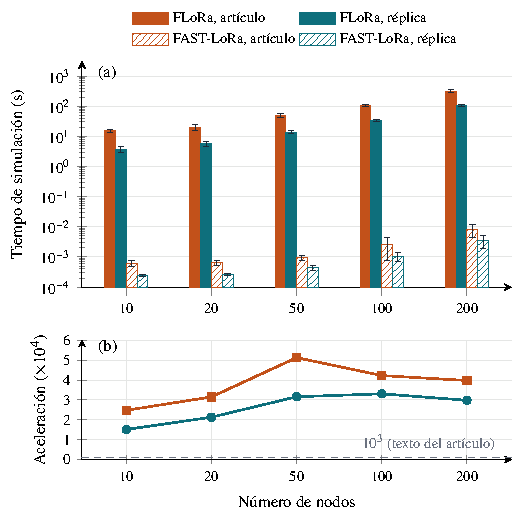
\includegraphics[width=\columnwidth]{../Figuras/fig6.pdf}
\caption{Tiempo de ejecución promedio sobre 1 a 5 gateways (a) y aceleración (b). En naranjo, los valores de la Fig.~6 de~\cite{fastlora}, leídos de los vectores del PDF; en verde azulado, la réplica, con 15 corridas por tamaño. Las barras de error son $\pm1$ desviación estándar. La línea punteada marca los $10^3$ que menciona el texto de~\cite{fastlora}.}
\label{fig:tiempos}
\end{figure}

La Fig.~\ref{fig:tiempos} compara los tiempos medidos con los de la Fig.~6 del artículo. En el portátil FLoRa pasa de 3,6~s con 10 nodos a 107~s con 200, y el modelo de 0,24 a 3,6~ms. Ambos son más rápidos que en el artículo, FLoRa de 3 a 4 veces y el modelo de 2 a 2,5 veces, algo esperable con un procesador más nuevo que el i5-8265U de los autores. En FLoRa la diferencia es mayor que la que explicaría la CPU, pero no se puede revisar porque el artículo no dice cómo se cronometró. La aceleración medida va de 1,5 a 3,3$\times10^4$, y la que se obtiene con los valores de la propia Fig.~6 va de 2,5 a 5,1$\times10^4$. El texto del artículo habla de hasta tres órdenes de magnitud, uno menos que lo que muestra su figura.

\subsection{Otras cifras del artículo}

Al recalcular las tablas aparecieron inconsistencias menores. El MAE de la EE del resumen (0,040) es el promedio sobre los nodos, y el del texto (0,038), el promedio de las 16 celdas de la Tabla~7. Las dos cifras son correctas, pero el artículo no aclara que miden cosas distintas. La desviación del error de la EE que da el texto, 0,068~bits/mJ, no sale de sus datos: el cuaderno de análisis de los autores calcula 0,0637, y 0,068 coincide con la raíz del error cuadrático medio, que incluye el sesgo. Por último, el texto llama a 200 nodos el escenario de mayor densidad evaluado, aunque la Tabla~6 llega a 500.

\section{Conclusiones y trabajo futuro}

La validación de FAST-LoRa se pudo repetir de forma exacta con el código y los datos de los autores, y sus Tablas~6 y~7 son correctas. Esas tablas, sin embargo, no separan el error del modelo del azar de FLoRa, que explica casi todo el error de la PDR que reportan. Con cinco corridas por red, el modelo coincide con FLoRa dentro del ruido en redes de hasta 100 nodos. Con 500 nodos subestima la PDR en 0,2 a 0,5$\times10^{-2}$, según cuántos parámetros se igualen. Para elegir configuraciones ese sesgo es pequeño, pero aparece justo donde la interferencia pesa, que es donde un modelo así haría más falta. En la EE, la diferencia entre ambas herramientas viene del tiempo en el aire y de la potencia de transmisión, y desaparece casi entera al igualarlos.

Para quien valide un modelo contra un simulador, una sola corrida no alcanza cuando el error buscado es del tamaño del ruido de muestreo. El piso~\eqref{eq:piso} se calcula en una línea y conviene reportarlo junto a cualquier MAE.

Quedan tres líneas de trabajo. La primera es encontrar la causa del sesgo con 500 nodos, comparando choque por choque los registros de FLoRa con las probabilidades del modelo. La segunda es repetir la validación con FLoRa oficial, sin los cambios de la fila~9 de la Tabla~\ref{tab:cabos}, y con el ADR encendido, que es como se usaría el modelo en la práctica; hoy el ADR del código publicado falla al ejecutarse. La tercera es contrastar ambos con mediciones en hardware, porque FLoRa también es un modelo y los parámetros de propagación de~\cite{bor} valen para un solo entorno. El código, los scripts y los datos derivados de este trabajo están en \url{https://github.com/KnDokusei/fastlora-replica}.

\begin{thebibliography}{99}
\bibitem{fastlora} L.~Acosta-García, J.~Aznar-Poveda, A.~J.~García-Sánchez \emph{et~al.}, ``FAST-LoRa: An efficient simulation framework for evaluating LoRaWAN networks and transmission parameter strategies,'' \emph{IEEE Access}, vol.~14, pp.~33518--33533, 2026.
\bibitem{flora} M.~Slabicki, G.~Premsankar y M.~Di~Francesco, ``Adaptive configuration of LoRa networks for dense IoT deployments,'' en \emph{Proc. IEEE/IFIP NOMS}, 2018.
\bibitem{abramson} N.~Abramson, ``The ALOHA system: Another alternative for computer communications,'' en \emph{Proc. AFIPS Fall Joint Computer Conf.}, 1970, pp.~281--285.
\bibitem{georgiou} O.~Georgiou y U.~Raza, ``Low power wide area network analysis: Can LoRa scale?'' \emph{IEEE Wireless Commun. Lett.}, vol.~6, no.~2, pp.~162--165, 2017.
\bibitem{bor} M.~C.~Bor, U.~Roedig, T.~Voigt y J.~M.~Alonso, ``Do LoRa low-power wide-area networks scale?'' en \emph{Proc. ACM MSWiM}, 2016, pp.~59--67.
\bibitem{magrin} D.~Magrin, M.~Centenaro y L.~Vangelista, ``Performance evaluation of LoRa networks in a smart city scenario,'' en \emph{Proc. IEEE ICC}, 2017.
\bibitem{vandenabeele} F.~Van~den~Abeele, J.~Haxhibeqiri, I.~Moerman y J.~Hoebeke, ``Scalability analysis of large-scale LoRaWAN networks in ns-3,'' \emph{IEEE Internet Things J.}, vol.~4, no.~6, pp.~2186--2198, 2017.
\bibitem{croce} D.~Croce, M.~Gucciardo, S.~Mangione, G.~Santaromita e I.~Tinnirello, ``Impact of LoRa imperfect orthogonality: Analysis of link-level performance,'' \emph{IEEE Commun. Lett.}, vol.~22, no.~4, pp.~796--799, 2018.
\bibitem{toro} V.~Toro-Betancur, G.~Premsankar, M.~Slabicki y M.~Di~Francesco, ``Modeling communication reliability in LoRa networks with device-level accuracy,'' en \emph{Proc. IEEE INFOCOM}, 2021.
\bibitem{zhang} X.~Zhang, Z.~Lin, S.~Gong, B.~Gu y D.~Niyato, ``Multiagent reinforcement learning with an attention mechanism for improving energy efficiency in LoRa networks,'' en \emph{Proc. IEEE GLOBECOM}, 2023, pp.~4152--4157.
\bibitem{liando} J.~C.~Liando, A.~Gamage, A.~W.~Tengourtius y M.~Li, ``Known and unknown facts of LoRa: Experiences from a large-scale measurement study,'' \emph{ACM Trans. Sensor Netw.}, vol.~15, no.~2, 2019.
\bibitem{lima} W.~G.~Lima \emph{et~al.}, ``LoRa technology propagation models for IoT network planning in the Amazon regions,'' \emph{Sensors}, vol.~24, no.~5, art.~1621, 2024.
\bibitem{repofast} jaznrp, ``FastLoRa,'' repositorio GitHub, commit \texttt{fb8b1be}. [En línea]. Disponible: \url{https://github.com/jaznrp/FastLoRa}
\bibitem{repomarltc} jaznrp, ``MultiAgent-MARLTC,'' repositorio GitHub, commits \texttt{d72e7ad} y \texttt{2f623b7}. [En línea]. Disponible: \url{https://github.com/jaznrp/MultiAgent-MARLTC}
\bibitem{repoflora} FLoRa, ``florasim/flora,'' repositorio GitHub, versión 1.1.0. [En línea]. Disponible: \url{https://github.com/florasim/flora}
\end{thebibliography}

\end{document}
